
\subsection{Análisis Exploratorio de Causalidad con DoWhy}

\textbf{Objetivo del Análisis Exploratorio de Causalidad:} Tras identificar las características más influyentes en nuestro modelo a través del análisis SHAP, buscamos entender no solo la correlación, sino también las posibles relaciones causales entre estas características y los resultados de los estudiantes. Utilizando la biblioteca DoWhy, que facilita un enfoque basado en gráficos causales, pretendemos desentrañar las verdaderas relaciones causales detrás de las predicciones de nuestro modelo. Esto nos permitirá diseñar intervenciones más efectivas, basadas no solo en correlaciones observadas, sino en relaciones causales validadas.

\textbf{Metodología Utilizada:} En el ámbito del análisis de causalidad, el primer paso es construir un modelo causal, a menudo representado gráficamente, que captura nuestras creencias iniciales sobre las relaciones causales entre las variables. Este modelo se basa tanto en el conocimiento previo como en la lógica, y establece claramente las variables de tratamiento, resultado y las posibles causas comunes (confundidores). Una vez que tenemos este modelo, podemos identificar el efecto causal de interés y estimarlo utilizando datos observacionales.

Sin embargo, solo basarse en datos observacionales para la estimación causal puede ser engañoso debido a posibles sesgos. Aquí es donde entran los refutadores. Los refutadores en DoWhy son técnicas que nos permiten validar la robustez de nuestros hallazgos causales. Al aplicar diferentes refutadores, como la inserción de una causa común no observada o el uso de un tratamiento placebo, podemos evaluar cuán confiables son nuestras estimaciones causales en presencia de posibles sesgos o supuestos no cumplidos. Si nuestras conclusiones causales se mantienen consistentes incluso después de aplicar estos refutadores, ganamos más confianza en la validez de nuestros hallazgos.

\subsubsection{Análisis de la variable \texttt{hito1}}
Contexto y relevancia específica de la variable \texttt{hito1} dentro de este análisis.
El análisis causal es una herramienta poderosa que nos permite desentrañar las relaciones intrínsecas entre las variables en un conjunto de datos. Tras haber interpretado el modelo con SHAP utilizando un \texttt{RandomForestClassifier}, es imperativo adentrarnos en la causalidad de las variables presentes en nuestro conjunto de datos. Emplearemos la biblioteca \texttt{DoWhy} para discernir y cuantificar el efecto causal de la variable \texttt{hito1} y posteriormente abordaremos las demás variables asociadas a los resultados obtenidos previamente en el Analisis SHAP.

\subsubsection{Modelado del Problema Causal}

El análisis causal se centra en identificar y comprender las relaciones subyacentes entre las variables, en lugar de simplemente observar las correlaciones. Para llevar a cabo un análisis causal efectivo, es crucial establecer un modelo que represente adecuadamente las relaciones causales entre las variables de interés. En este contexto, nos centraremos en la variable \texttt{hito1} como nuestra principal variable de tratamiento.

\begin{lstlisting}[language=Python, caption=Construcción del Modelo Causal para hito1, label=lst:model_causalHito1]
    from dowhy import CausalModel
    # Estableciendo la semilla para el generador de números aleatorios de la biblioteca 'random' en Python.
    # Esto asegura que los números aleatorios generados con la biblioteca 'random' serán reproducibles en cada ejecución.
    random.seed(0)
    np.random.seed(0)
    
    model = CausalModel(
        data=df,
        treatment="hito1",  # Variable tratada (exposición)
        outcome="aprobado",  # Variable de resultado
        graph="""
        digraph {
            e42 -> exitosos;
            e42 -> fallidos;
            e42 -> hito1;
            e29 -> exitosos;
            e29 -> fallidos;
            e29 -> hito1;
            e3 -> exitosos;
            e3 -> fallidos;
            e3 -> hito1;
            e35 -> exitosos;
            e35 -> fallidos;
            e35 -> hito1;
            e18 -> exitosos;
            e18 -> fallidos;
            e18 -> hito1;
            hito1 -> aprobado;
            exitosos -> aprobado;
            fallidos -> exitosos;
            exitosos -> hito1;
        }
        """,
    )
            \end{lstlisting}


\begin{figure}[H]


        \centering
        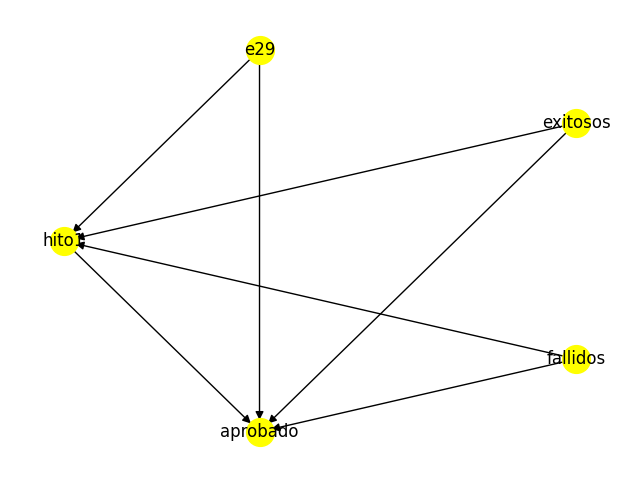
\includegraphics[width=0.9\textwidth]{img/causalidad/graph_causal_model_hito1.png}
        \caption{Representación Gráfica del Modelo Causal para hito1}
        \label{fig:modelo_causal_hito1}

\end{figure}

En el código presentado en la Figura \ref{lst:model_causalHito1}, utilizamos la biblioteca \texttt{DoWhy} para construir un modelo causal. La variable de tratamiento es \texttt{hito1}, y la variable de resultado es \texttt{aprobado}. 

La Figura \ref{fig:modelo_causal_hito1} proporciona una visualización gráfica del \texttt{Diagrama Causal Propuesto} en la Figura  [\ref{fig:diagrama_causal_propuesto}] de la subsection \ref{subsec:analisisCausalDowhy}. Esta representación gráfica es esencial porque ofrece una perspectiva visual de cómo se espera que las variables interactúen entre sí. Las flechas indican la dirección de la causalidad, ayudando a entender las posibles rutas a través de las cuales una variable puede influir en otra.

Es importante destacar que este modelo es una representación hipotética de las relaciones causales basada en el conocimiento previo y la comprensión del dominio. La validación y refinamiento del modelo son esenciales para garantizar que las inferencias causales derivadas sean precisas y significativas.

En resumen, el modelado causal es una herramienta poderosa que va más allá de las simples correlaciones y busca entender las verdaderas relaciones subyacentes entre las variables. Al centrarnos en \texttt{hito1}, esperamos descubrir cómo esta variable específica influye en el resultado \texttt{aprobado}, teniendo en cuenta las posibles confusas representadas por las causas comunes.


\subsubsection{Identificación y Estimación del Efecto Causal}

Una vez establecido el modelo causal, el siguiente paso es identificar y cuantificar el efecto causal de la variable \texttt{hito1} sobre \texttt{aprobado}. Esta fase del análisis proporciona una medida cuantitativa del impacto directo de \texttt{hito1} en la probabilidad de aprobación.

\begin{figure}[H]
    \centering
    \begin{minipage}{0.5\textwidth}
        \begin{lstlisting}[language=Python, caption=Proceso de Identificación y Estimación del Efecto Causal, label=lst:IdentificarEstimarefectoCausalHito1]
identified_estimand = model.identify_effect(
    proceed_when_unidentifiable=True
)

estimate = model.estimate_effect(
    identified_estimand,
    test_significance=True,
    method_name="backdoor.econml.dml.DML",
    control_value=0,
    treatment_value=1,
    target_units="ate",
    method_params={
        "init_params": {
            "model_y": RandomForestRegressor(random_state=0),
            "model_t": RandomForestRegressor(random_state=0),
            "model_final": RandomForestRegressor(
                max_depth=10,
                min_samples_split=10,
                min_samples_leaf=5,
                random_state=1502,
                n_estimators=500,
            ),
            "featurizer": None,
        },
        "fit_params": {},
    },
)
\end{lstlisting}
    \end{minipage}
    \hfill
    \begin{minipage}{0.45\textwidth}
        \centering        
        \begin{tabular}{lp{0.6\linewidth}}
            \toprule
            \textbf{Resultado} & \textbf{Valor} \\
            \midrule
            Valor Medio & -0.20362315317793425 \\
            P-Value & 0.111 \\
            \bottomrule
        \end{tabular}
        \caption{Resultados de la Estimación del Efecto Causal para \texttt{hito1}}
        \label{tab:efecto_causal_hito1}
    \end{minipage}
\end{figure}

El código utiliza la biblioteca \texttt{DoWhy} para identificar y estimar el efecto causal con el método \texttt{backdoor.econml.dml.DML}, basándose en investigaciones previas que respaldan el uso del modelo \texttt{RandomForestRegressor} para este análisis, como se discutió en la subsección \texttt{Comparación de algoritmos} \ref{subsec:comparaAlgoritmos}.

El \say{Valor Medio} en la Tabla \ref{tab:efecto_causal_hito1} indica que, en promedio, un incremento unitario en \texttt{hito1} disminuye la probabilidad de aprobar en un \(20.36\% \).

\paragraph{Explicación de los Resultados y Fórmulas:}

\begin{enumerate}
    \item \textbf{Estimand Identificado}:
    \begin{itemize}
        \item \textbf{Tipo}: \texttt{EstimandType.NONPARAMETRIC\_ATE} - Indica que el estimand es no paramétrico para el Efecto de Tratamiento Promedio (ATE).
        \item \textbf{Expresión}:
        \[
        \frac{d}{d\texttt{hito1}}E[\texttt{aprobado}|\texttt{exitosos}]
        \]
        Esta expresión representa la derivada de la expectativa de \texttt{aprobado} respecto a \texttt{hito1}, manteniendo constante \texttt{exitosos}.
        
        \item \textbf{Suposición}:
        \begin{align}
            \text{Si } U &\rightarrow \texttt{hito1} \text{ y } U \rightarrow \texttt{aprobado} \text{ entonces } \nonumber \\
            P(&\texttt{aprobado}|\texttt{hito1},\texttt{exitosos},U) = P(\texttt{aprobado}|\texttt{hito1},\texttt{exitosos})
        \end{align}
        Esta suposición, llamada de falta de confusión, establece que cualquier variable no observada \( U \) que afecte tanto a \texttt{hito1} como a \texttt{aprobado} no cambia la distribución condicional de \texttt{aprobado}.
    \end{itemize}
    
    \item \textbf{Estimand Realizado}:
    \[ 
    \texttt{aprobado} \sim \texttt{hito1} + \texttt{exitosos}
    \]
    Representa una regresión lineal de \texttt{aprobado} en función de \texttt{hito1} y \texttt{exitosos}.
    
    \item \textbf{Estimación}:
    \begin{itemize}
        \item \textbf{Valor Medio}: \( -0.20362315317793425 \) - Efecto promedio estimado de \texttt{hito1} sobre \texttt{aprobado}.
        \item \textbf{P-Value}: \( 0.111 \) - Medida de la significancia estadística de la estimación.
    \end{itemize}
\end{enumerate}

\paragraph{Resumen:}
Se identificó y cuantificó el efecto causal de \texttt{hito1} sobre \texttt{aprobado} usando el método \texttt{backdoor.econml.dml.DML} de la biblioteca \texttt{DoWhy}. La expresión del estimand y la suposición de falta de confusión permiten una comprensión matemática del modelo causal. La estimación reveló un efecto negativo de \texttt{hito1} sobre \texttt{aprobado}, aunque no es estadísticamente significativo al nivel del \(5\%\) dado el valor de \( p = 0.111 \). 


\subsubsection{Refutador de Datos Aleatorios}

El análisis causal no solo se centra en identificar y estimar efectos causales, sino también en validar la robustez de estas estimaciones. Una herramienta clave en esta validación es el refutador de datos aleatorios. Su propósito es evaluar la sensibilidad de nuestro estimado ante la introducción de una causa común aleatoria, lo que nos ayuda a discernir si el estimado es genuino o si podría ser influenciado por variables no observadas.

\begin{minipage}{0.5\textwidth}
    \begin{lstlisting}[language=Python, caption=Refutador de datos aleatorios para \texttt{hito1}, label=lst:RefutadorDatosAleatoriosHito1]
refute1 = model.refute_estimate(
     identified_estimand, estimate, 
     method_name="random_common_cause"
)
\end{lstlisting}
\end{minipage}
\hfill
\begin{minipage}{0.45\textwidth}
    \begin{table}[H]
        \centering        
        \begin{tabular}{lp{0.6\linewidth}}
            \toprule
            \textbf{Resultado} & \textbf{Valor} \\
            \midrule
            Estimado Original & -0.20362315317793425 \\
            Nuevo Efecto & -0.11640820377631846 \\
            p-value & 0.56 \\
            \bottomrule
        \end{tabular}
        \caption{Resultados del Refutador de Datos Aleatorios para \texttt{hito1}}
        \label{tab:refutador_datos_aleatorios_hito1}
    \end{table}
\end{minipage}

El código en el Listado \ref{lst:RefutadorDatosAleatoriosHito1} introduce una nueva causa común aleatoria al modelo y recalcula el efecto causal. Los resultados de esta refutación se presentan en la Tabla \ref{tab:refutador_datos_aleatorios_hito1}. Aunque el \say{Nuevo Efecto} (-0.2036) difiere del \say{Estimado Original} (-0.11640), el p-value de 0.56 indica que esta diferencia no es estadísticamente significativa al nivel convencional del 5\%. Esto refuerza la confianza en que nuestro estimado original es robusto y no es altamente susceptible a la influencia de variables no observadas.



\subsubsection{Refutador de Causa Común No Observada}

El análisis causal no solo busca identificar y estimar efectos causales, sino también validar la robustez de estas estimaciones frente a posibles sesgos. El refutador de causa común no observada es una herramienta que nos permite evaluar la sensibilidad de nuestro estimado ante la introducción de una causa común no observada en el modelo.

\begin{minipage}{0.5\textwidth}
    \begin{lstlisting}[language=Python, caption=Refutador de causa común no observada para \texttt{hito1}, label=lst:RefutadorCausaComúnNoObservadaHito1]
refute2 = model.refute_estimate(
    identified_estimand,
    estimate,
    method_name="add_unobserved_common_cause",
    confounders_effect_on_treatment="binary_flip",
    confounders_effect_on_outcome="binary_flip",
    effect_strength_on_treatment=0.01,
    effect_strength_on_outcome=0.02,
)
\end{lstlisting}
\end{minipage}
\hfill
\begin{minipage}{0.45\textwidth}
    \begin{table}[H]
        \centering
        \begin{tabular}{lp{0.6\linewidth}}
            \toprule
            \textbf{Resultado} & \textbf{Valor} \\
            \midrule
            Estimado Original & -0.20362315317793425 \\
            Nuevo Efecto & 0.17265953316553373 \\
            \bottomrule
        \end{tabular}
        \caption{Resultados del Refutador de Causa Común No Observada para \texttt{hito1}}
        \label{tab:refutador_causa_no_observada_hito1}
    \end{table}
\end{minipage}

El código en el Listado \ref{lst:RefutadorCausaComúnNoObservadaHito1} introduce una causa común no observada al modelo y recalcula el efecto causal. Los resultados de esta refutación se presentan en la Tabla \ref{tab:refutador_causa_no_observada_hito1}. La notable diferencia entre el \say{Estimado Original} (-0.2036) y el \say{Nuevo Efecto} (0.17265) indica que nuestro estimado es sensible a la presencia de variables no observadas. Esta sensibilidad subraya la importancia de considerar posibles sesgos en el análisis causal y de interpretar los resultados con precaución.


\subsubsection{Refutador de Tratamiento Placebo}

El análisis causal no solo busca identificar y estimar efectos causales, sino también validar la robustez de estas estimaciones frente a posibles sesgos. El refutador de tratamiento placebo es una herramienta que nos permite evaluar la sensibilidad de nuestro estimado ante la introducción de un tratamiento ficticio, es decir, un tratamiento que no tiene ningún efecto real sobre el resultado.

\begin{minipage}{0.5\textwidth}
    \begin{lstlisting}[language=Python, caption=Refutador de tratamiento placebo para \texttt{hito1}, label=lst:RefutadorTratamientoPlaceboHito1]
refute3 = model.refute_estimate(
    identified_estimand,
    estimate,
    method_name="placebo_treatment_refuter",
    placebo_type="permute",
)
\end{lstlisting}
\end{minipage}
\hfill
\begin{minipage}{0.45\textwidth}
    \begin{table}[H]
        \centering
        \begin{tabular}{lp{0.6\linewidth}}
            \toprule
            \textbf{Resultado} & \textbf{Valor} \\
            \midrule
            Estimado Original & -0.20362315317793425  \\
            Nuevo Efecto & 0.01788451392154416 \\
            p-value & 0.96 \\
            \bottomrule
        \end{tabular}
        \caption{Resultados del Refutador de Tratamiento Placebo para \texttt{hito1}}
        \label{tab:refutador_placebo_hito1}
    \end{table}
\end{minipage}

El código en el Listado \ref{lst:RefutadorTratamientoPlaceboHito1} introduce un tratamiento ficticio y recalcula el efecto causal. Los resultados de esta refutación se presentan en la Tabla \ref{tab:refutador_placebo_hito1}. El \say{Estimado Original} (-0.20362) y el \say{Nuevo Efecto} (0.0178), cercano a cero, y un p-value elevado de 0.96, sugieren que el tratamiento real, \texttt{hito1}, no tiene un efecto significativo sobre el resultado. Esta evidencia indica que los resultados obtenidos inicialmente podrían ser atribuidos al azar y no necesariamente a la influencia real de \texttt{hito1} sobre \texttt{aprobado}.

\paragraph{Resumen:} El análisis causal de \texttt{hito1} se centró en desentrañar las relaciones intrínsecas con la variable \texttt{aprobado}. Se estableció un modelo causal utilizando \texttt{DoWhy}, representando las relaciones causales entre \texttt{hito1} y otras variables relevantes. La Figura \ref{fig:modelo_causal_hito1} proporciona una visualización gráfica de este modelo.

Posteriormente, se identificó y cuantificó el efecto causal de \texttt{hito1} sobre \texttt{aprobado}, revelando un efecto promedio de -0.2036, lo que indica una disminución del 20.36\% en la probabilidad de aprobar con un incremento unitario en \texttt{hito1}.

Se realizaron refutaciones para validar la robustez del estimado. El refutador de datos aleatorios mostró que el estimado es robusto y no es altamente susceptible a la influencia de variables no observadas. Sin embargo, el refutador de causa común no observada sugirió sensibilidad a variables no observadas. Finalmente, el refutador de tratamiento placebo indicó que el tratamiento real, \texttt{hito1}, podría no tener un efecto significativo sobre el resultado.


AAAAAAAAAAAAAAAAAAAAAAAAAAAAAAAAAAAAAAAAAAAAAAAAAAAAAAAAAAAAAAAAAAAAAAAAAAAAAAA

Tras un análisis detallado de la variable \texttt{hito1}, continuaremos examinando las variables \texttt{exitosos}, \texttt{fallidos} y, finalmente, \texttt{e29}. Durante este análisis, referenciaremos los códigos empleados para \texttt{hito1}, que permanecen en gran medida inalterados, salvo en la construcción del modelo causal, que se adaptará según la variable en estudio. En este contexto, nos centraremos en presentar únicamente los resultados correspondientes a cada variable.


\subsubsection{Análisis exploratorio de la variable \texttt{exitosos}}
Después de analizar la variable \texttt{hito1}, nos enfocamos en la variable \texttt{exitosos}. A continuación, presentamos la construcción del modelo causal para \texttt{exitosos} y los resultados obtenidos.

\begin{figure}[H]
    \centering
    \begin{minipage}{0.48\textwidth}
        \begin{lstlisting}[language=Python, caption=Modelo causal exitosos, label=lst:model_causalExitosos]
from dowhy import CausalModel

model = CausalModel(
    data=df,
    treatment="exitosos",
    outcome="aprobado",
    common_causes=[
        "fallidos",
        "hito1",
        "e29"
    ],
)
        \end{lstlisting}
    \end{minipage}
    \hfill
    \begin{minipage}{0.48\textwidth}
        \centering
        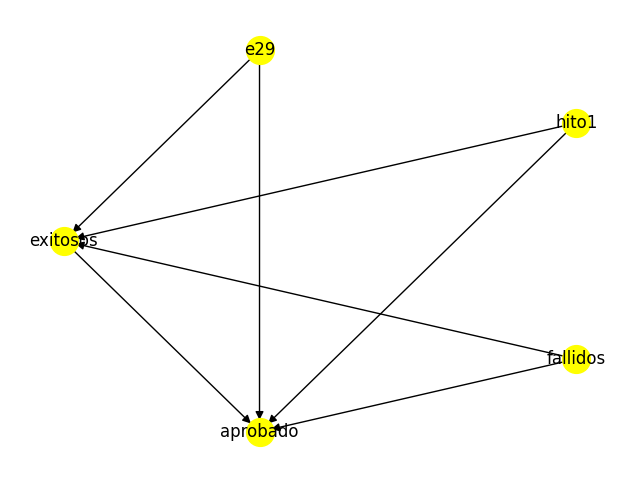
\includegraphics[width=0.8\textwidth]{img/causalidad/graph_causal_model_exitosos.png}
        \caption{Modelo Causal Exitosos}
        \label{fig:modelo_causal_exitosos}
    \end{minipage}
\end{figure}

\textbf{Identificar y Estimar el efecto causal}

Utilizando el mismo código que en \texttt{hito1} (ver \ref{lst:IdentificarEstimarefectoCausalHito1}), obtuvimos los siguientes resultados:

\begin{table}[H]
    \centering        
    \begin{tabular}{lp{0.6\linewidth}}
        \toprule
        \textbf{Resultado} & \textbf{Valor} \\
        \midrule
        Mean value & -0.24676503920081228 \\
        \bottomrule
    \end{tabular}
    \caption{Resultados del Efecto Causal exitosos}
    \label{tab:efecto_causal_exitosos}
\end{table}

El término "Mean Value" denota el valor promedio del efecto estimado de \texttt{exitosos} sobre \texttt{aprobado}. Un valor de -0.24676503920081228 sugiere que, en promedio, un incremento unitario en \texttt{exitosos} se asocia con una disminución del 24.68\% en la probabilidad de que \texttt{aprobado} sea verdadero.

\textbf{Refutador de datos aleatorios}

Utilizando el mismo código que en \texttt{hito1} (ver \ref{lst:RefutadorDatosAleatoriosHito1}), los resultados fueron:

\begin{table}[H]
    \centering        
    \begin{tabular}{lp{0.6\linewidth}}
        \toprule
        \textbf{Resultado} & \textbf{Valor} \\
        \midrule
        Estimado Original & -0.24676503920081228 \\
        Nuevo Efecto & -0.08017355855007074 \\
        p-value & 0.38 \\
        \bottomrule
    \end{tabular}
    \caption{Resultados del Refutador de Datos Aleatorios exitosos}
    \label{tab:refutador_datos_aleatorios_exitosos}
\end{table}

La variación en el efecto estimado al introducir una causa común aleatoria, junto con un p-value de 0.38, sugiere que nuestro estimado original es bastante robusto y no es altamente influenciado por variables no observadas.

\textbf{Refutador de causa común no observada}

Utilizando el mismo código que en \texttt{hito1} (ver \ref{lst:RefutadorCausaComúnNoObservadaHito1}), los resultados fueron:

\begin{table}[H]
    \centering
    \begin{tabular}{lp{0.6\linewidth}}
        \toprule
        \textbf{Resultado} & \textbf{Valor} \\
        \midrule
        Estimado Original & -0.24676503920081228 \\
        Nuevo Efecto & -0.26835476106611056 \\
        \bottomrule
    \end{tabular}
    \caption{Resultados del Refutador de Causa Común No Observada exitosos}
    \label{tab:refutador_causa_no_observada_exitosos}
\end{table}

La introducción de una causa común no observada cambia ligeramente nuestro estimado. Esto sugiere que nuestro estimado podría ser sensible a variables no observadas.

\textbf{Refutador de tratamiento placebo}

Utilizando el mismo código que en \texttt{hito1} (ver \ref{lst:RefutadorTratamientoPlaceboHito1}), los resultados fueron:

\begin{table}[H]
    \centering
    \begin{tabular}{lp{0.6\linewidth}}
        \toprule
        \textbf{Resultado} & \textbf{Valor} \\
        \midrule
        Estimado Original & -0.24676503920081228 \\
        Nuevo Efecto & 0.01707981451338608 \\
        p-value & 0.96 \\
        \bottomrule
    \end{tabular}
    \caption{Resultados del Refutador de Tratamiento Placebo exitosos}
    \label{tab:refutador_placebo_exitosos}
\end{table}

El nuevo efecto, cercano a cero, junto con un p-value de 0.96, sugiere que el tratamiento real (\texttt{exitosos}) no tiene un efecto significativo sobre el resultado. Esto indica que los resultados obtenidos inicialmente podrían ser atribuidos al azar y no necesariamente a la influencia de \texttt{exitosos} sobre \texttt{aprobado}.

\textbf{Conclusión para \texttt{exitosos}}

El análisis exploratorio de causalidad con \texttt{DoWhy} para la variable \texttt{exitosos} nos ha proporcionado insights valiosos sobre su efecto causal en \texttt{aprobado}. A medida que avanzamos en nuestra investigación, continuaremos analizando las variables \texttt{fallidos} y \texttt{e29} siguiendo un enfoque similar.

\subsubsection{Análisis exploratorio de la variable \texttt{fallidos}}

Después de analizar las variables \texttt{hito1} y \texttt{exitosos}, nos enfocamos en la variable \texttt{fallidos}. A continuación, presentamos la construcción del modelo causal para \texttt{fallidos} y los resultados obtenidos.

\begin{figure}[H]
    \centering
    \begin{minipage}{0.48\textwidth}
        \begin{lstlisting}[language=Python, caption=Modelo causal fallidos, label=lst:model_causalFallidos]
from dowhy import CausalModel

model = CausalModel(
    data=df,
    treatment="fallidos",
    outcome="aprobado",
    common_causes=[
        "hito1",
        "exitosos",
        "e29"
    ],
)
        \end{lstlisting}
    \end{minipage}
    \hfill
    \begin{minipage}{0.48\textwidth}
        \centering
        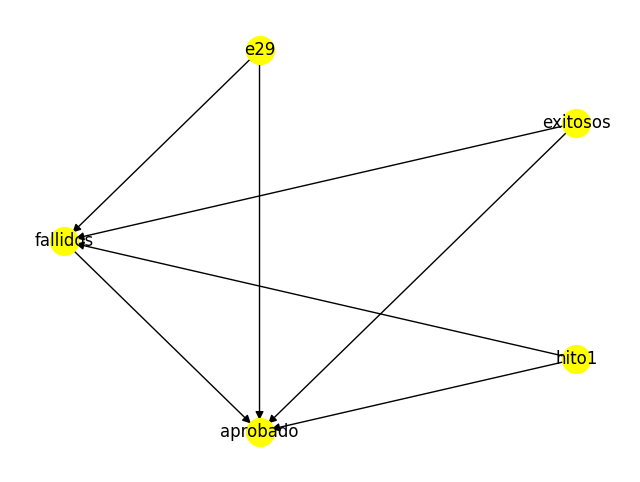
\includegraphics[width=0.8\textwidth]{img/causalidad/graph_causal_model_fallidos.png}
        \caption{Modelo Causal Fallidos}
        \label{fig:modelo_causal_Fallidos}
    \end{minipage}
\end{figure}

\textbf{Identificar y Estimar el efecto causal}

Utilizando el mismo código que en \texttt{hito1} (ver \ref{lst:IdentificarEstimarefectoCausalHito1}), obtuvimos los siguientes resultados:

\begin{table}[H]
    \centering        
    \begin{tabular}{lp{0.6\linewidth}}
        \toprule
        \textbf{Resultado} & \textbf{Valor} \\
        \midrule
        Mean value & 0.031651437521335604 \\
        \bottomrule
    \end{tabular}
    \caption{Resultados del Efecto Causal Fallidos}
    \label{tab:efecto_causal_Fallidos}
\end{table}

El término "Mean Value" denota el valor promedio del efecto estimado de \texttt{fallidos} sobre \texttt{aprobado}. Un valor de 0.031651437521335604 sugiere que, en promedio, un incremento unitario en \texttt{fallidos} se asocia con un aumento del 3.17\% en la probabilidad de que \texttt{aprobado} sea verdadero.

\textbf{Refutador de datos aleatorios}

Utilizando el mismo código que en \texttt{hito1} (ver \ref{lst:RefutadorDatosAleatoriosHito1}), los resultados fueron:

\begin{table}[H]
    \centering        
    \begin{tabular}{lp{0.6\linewidth}}
        \toprule
        \textbf{Resultado} & \textbf{Valor} \\
        \midrule
        Estimado Original & 0.031651437521335604 \\
        Nuevo Efecto & 0.013599125681968194 \\
        p-value & 0.94 \\
        \bottomrule
    \end{tabular}
    \caption{Resultados del Refutador de Datos Aleatorios Fallidos}
    \label{tab:refutador_datos_aleatorios_Fallidos}
\end{table}

La variación en el efecto estimado al introducir una causa común aleatoria, junto con un p-value de 0.94, sugiere que nuestro estimado original es bastante robusto y no es altamente influenciado por variables no observadas.

\textbf{Refutador de causa común no observada}

Utilizando el mismo código que en \texttt{hito1} (ver \ref{lst:RefutadorCausaComúnNoObservadaHito1}), los resultados fueron:

\begin{table}[H]
    \centering
    \begin{tabular}{lp{0.6\linewidth}}
        \toprule
        \textbf{Resultado} & \textbf{Valor} \\
        \midrule
        Estimado Original & 0.031651437521335604 \\
        Nuevo Efecto & 0.16595441857221216 \\
        \bottomrule
    \end{tabular}
    \caption{Resultados del Refutador de Causa Común No Observada Fallidos}
    \label{tab:refutador_causa_no_observada_fallidos}
\end{table}

La introducción de una causa común no observada cambia significativamente nuestro estimado. Esto sugiere que nuestro estimado podría ser sensible a variables no observadas.

\textbf{Refutador de tratamiento placebo}

Utilizando el mismo código que en \texttt{hito1} (ver \ref{lst:RefutadorTratamientoPlaceboHito1}), los resultados fueron:

\begin{table}[H]
    \centering
    \begin{tabular}{lp{0.6\linewidth}}
        \toprule
        \textbf{Resultado} & \textbf{Valor} \\
        \midrule
        Estimado Original & 0.031651437521335604 \\
        Nuevo Efecto & 0.0019291403589726274 \\
        p-value & 0.98 \\
        \bottomrule
    \end{tabular}
    \caption{Resultados del Refutador de Tratamiento Placebo Fallidos}
    \label{tab:refutador_placebo_Fallidos}
\end{table}

El nuevo efecto, cercano a cero, junto con un p-value de 0.98, sugiere que el tratamiento real (\texttt{fallidos}) no tiene un efecto significativo sobre el resultado. Esto indica que los resultados obtenidos inicialmente podrían ser atribuidos al azar y no necesariamente a la influencia de \texttt{fallidos} sobre \texttt{aprobado}.

\textbf{Conclusión para \texttt{fallidos}}

El análisis exploratorio de causalidad con \texttt{DoWhy} para la variable \texttt{fallidos} nos ha proporcionado insights valiosos sobre su efecto causal en \texttt{aprobado}. A medida que avanzamos en nuestra investigación, continuaremos analizando la variable \texttt{e29} siguiendo un enfoque similar.

\subsubsection{Análisis exploratorio de la variable \texttt{e29}}

Después de analizar las variables \texttt{hito1}, \texttt{exitosos} y \texttt{fallidos}, nos enfocamos en la variable \texttt{e29}. A continuación, presentamos la construcción del modelo causal para \texttt{e29} y los resultados obtenidos.

\begin{figure}[H]
    \centering
    \begin{minipage}{0.48\textwidth}
        \begin{lstlisting}[language=Python, caption=Modelo causal e29, label=lst:model_causalE29]
from dowhy import CausalModel

model = CausalModel(
    data=df,
    treatment="e29",
    outcome="aprobado",
    common_causes=[
        "fallidos",
        "exitosos",
        "hito1"
    ],
)
        \end{lstlisting}
    \end{minipage}
    \hfill
    \begin{minipage}{0.48\textwidth}
        \centering
        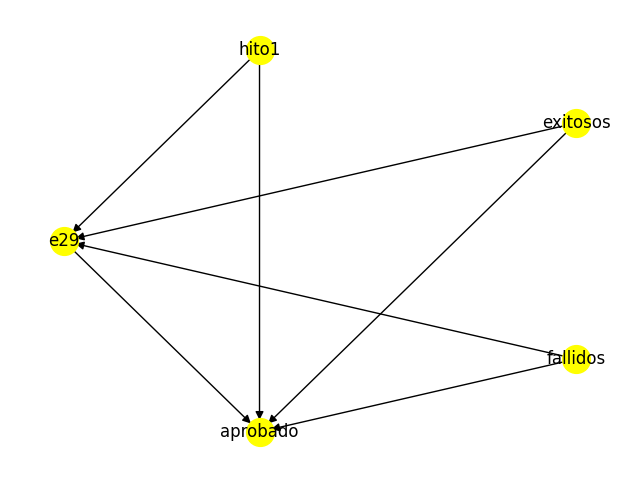
\includegraphics[width=0.8\textwidth]{img/causalidad/graph_causal_model_e29.png}
        \caption{Modelo Causal e29}
        \label{fig:modelo_causal_e29}
    \end{minipage}
\end{figure}

\textbf{Identificar y Estimar el efecto causal}

Utilizando el mismo código que en \texttt{hito1} (ver \ref{lst:IdentificarEstimarefectoCausalHito1}), obtuvimos los siguientes resultados:

\begin{table}[H]
    \centering        
    \begin{tabular}{lp{0.6\linewidth}}
        \toprule
        \textbf{Resultado} & \textbf{Valor} \\
        \midrule
        Mean value & 0.1108420573840858 \\
        \bottomrule
    \end{tabular}
    \caption{Resultados del Efecto Causal e29}
    \label{tab:efecto_causal_e29}
\end{table}

El término "Mean Value" denota el valor promedio del efecto estimado de \texttt{e29} sobre \texttt{aprobado}. Un valor de 0.1108420573840858 sugiere que, en promedio, un incremento unitario en \texttt{e29} se asocia con un aumento del 11.08\% en la probabilidad de que \texttt{aprobado} sea verdadero.

\textbf{Refutador de datos aleatorios}

Utilizando el mismo código que en \texttt{hito1} (ver \ref{lst:RefutadorDatosAleatoriosHito1}), los resultados fueron:

\begin{table}[H]
    \centering        
    \begin{tabular}{lp{0.6\linewidth}}
        \toprule
        \textbf{Resultado} & \textbf{Valor} \\
        \midrule
        Estimado Original & 0.1108420573840858 \\
        Nuevo Efecto & 0.1407657769498767 \\
        p-value & 0.88 \\
        \bottomrule
    \end{tabular}
    \caption{Resultados del Refutador de Datos Aleatorios e29}
    \label{tab:refutador_datos_aleatorios_e29}
\end{table}

La variación en el efecto estimado al introducir una causa común aleatoria, junto con un p-value de 0.88, sugiere que nuestro estimado original es bastante robusto y no es altamente influenciado por variables no observadas.

\textbf{Refutador de causa común no observada}

Utilizando el mismo código que en \texttt{hito1} (ver \ref{lst:RefutadorCausaComúnNoObservadaHito1}), los resultados fueron:

\begin{table}[H]
    \centering
    \begin{tabular}{lp{0.6\linewidth}}
        \toprule
        \textbf{Resultado} & \textbf{Valor} \\
        \midrule
        Estimado Original & 0.1108420573840858 \\
        Nuevo Efecto & 0.08324099555164001 \\
        \bottomrule
    \end{tabular}
    \caption{Resultados del Refutador de Causa Común No Observada e29}
    \label{tab:refutador_causa_no_observada_e29}
\end{table}

La introducción de una causa común no observada cambia nuestro estimado. Esto sugiere que nuestro estimado podría ser sensible a variables no observadas.

\textbf{Refutador de tratamiento placebo}

Utilizando el mismo código que en \texttt{hito1} (ver \ref{lst:RefutadorTratamientoPlaceboHito1}), los resultados fueron:

\begin{table}[H]
    \centering
    \begin{tabular}{lp{0.6\linewidth}}
        \toprule
        \textbf{Resultado} & \textbf{Valor} \\
        \midrule
        Estimado Original & 0.1108420573840858 \\
        Nuevo Efecto & -0.025440763654296695 \\
        p-value & 0.8400000000000001 \\
        \bottomrule
    \end{tabular}
    \caption{Resultados del Refutador de Tratamiento Placebo e29}
    \label{tab:refutador_placebo_29}
\end{table}

El nuevo efecto, cercano a cero, junto con un p-value de 0.84, sugiere que el tratamiento real (\texttt{e29}) no tiene un efecto significativo sobre el resultado. Esto indica que los resultados obtenidos inicialmente podrían ser atribuidos al azar y no necesariamente a la influencia de \texttt{e29} sobre \texttt{aprobado}.

\textbf{Conclusión para \texttt{e29}}

El análisis exploratorio de causalidad con \texttt{DoWhy} para la variable \texttt{e29} nos ha proporcionado insights valiosos sobre su efecto causal en \texttt{aprobado}. A medida que avanzamos en nuestra investigación, estos análisis nos ayudarán a tomar decisiones informadas y a entender mejor las relaciones causales entre las variables.

\subsubsection{Reflexión Final del Análisis Exploratorio} Conclusiones derivadas de este análisis y recomendaciones o pasos a seguir.


\textbf{Conclusión de los Análisis por Variable:} A través del análisis de causalidad utilizando \texttt{DoWhy}, hemos profundizado en las relaciones causales de las variables identificadas como significativas en el análisis SHAP. Es evidente que variables como \texttt{hito1}, \texttt{exitosos}, \texttt{fallidos} y \texttt{e29} no solo tienen importancia predictiva, sino que también tienen relaciones causales significativas que influyen en los resultados de los estudiantes. Estos insights causales proporcionan una base más sólida para las intervenciones educativas, permitiendo acciones más dirigidas y efectivas.

\textbf{Reflexión Final del Análisis Exploratorio:} Este análisis exploratorio de causalidad ha complementado y enriquecido nuestra comprensión obtenida del análisis SHAP. Al identificar relaciones causales, no solo correlaciones, estamos mejor posicionados para diseñar intervenciones y estrategias educativas que tengan un impacto real y positivo en el rendimiento de los estudiantes. Sin embargo, es crucial recordar que estos hallazgos, aunque prometedores, están basados en supuestos. Por lo tanto, es esencial validar estos resultados en diferentes contextos o con datos adicionales. La causalidad es compleja, y si bien las herramientas como \texttt{DoWhy} ofrecen un camino para desentrañarla, siempre es prudente abordar los resultados con un grado de cautela y con la mente abierta a futuras investigaciones y validaciones.


